\chapter*{Wprowadzenie}
% jaka będzie wartość dodana tego co zrobimy
% cała ścieżka Informatyka -> nasza praca
% celem naszym było usystematyzować pracę nad systemami dla sumerologów

% nasza ścieżka: Informatyka -> Inżynieria oprogramowania -> różne podejścia -> domain-specific podejście -> domain specific language

% 1. krótki opis problemu - są sumerolodzy, mają tabliczki, chcą sprawnie wyszukiwać
% Problem wyszukiwania tabliczek sumeryjskich był wiele razy podejmowany na naszym wydziale.
Dawno dawno temu żyli sobie sumerowie, którzy produkowali ogromne ilości tabliczek. Były to głównie teksty gospodarcze (rozliczenia itp). Wiele z nich po jakimś czasie stała się bezużyteczna - wyrzucano je lub korzystano z nich przy budowie dróg itp. Archeolodzy znaleźli sporo takich tabliczek, w dużej mierze zniszczonych i w ogóle. Część z nich wrzucili do komputera w formie cyfrowej. Największa baza danych zawierających takie tabliczki to CDLI - zawiera ich prawie 225 tys.
% Istnieje wiele baz danych zawierających teksty odczytane z tabliczek sumeryjskich (najbardziej znana - CDLI zawiera ich prawie 225 tys.). 
Na podstawie tych tabliczek można wiele dowiedzieć się o życiu zwykłych ludzi, o wypłatach, zasiłkach i dniach wolnych. Takie informacje próbują z tabliczek wyciągnąć sumerolodzy.
% Sumerolodzy zajmują się badaniem i przetwarzaniem tych tekstów, 
Jednak wyszukiwanie interesujących ich tabliczek jest dosyć niewygodne. Wynika to przede wszystkim z nieznajomości specyficznych dla baz danych języków zapytań. 
Większość serwisów internetowych udostępnia formularze ułatwiające wprowadzanie kryteriów wyszukiwania, jednakże mają one ograniczone możliwości (nie pozwalają na skomplikowane konstrukcje). Dlatego istnieje potrzeba stworzenia narzędzia, które będzie łączyło w sobie jak największą siłę wyrazu i łatwość użycia przez osoby znające jedynie dziedzinę problemu. A my chcemy pomóc!!

% 2. różne podejścia do tworzenia oprogramowania
Rozwiązywaniem tego typu problemów zajmuje się informatyka poprzez tworzenie odpowiednich systemów. Powstało wiele różnych systemów i na tej podstawie wytworzyły się różne podejścia. Zrobiło się takie kółko: powstają systemy - ludzie coś zauważają - powstają nowe podejścia - ludzie ich używają - powstają systemy
% Część z nich rozważałyśmy zastanawiająć się nad problemem sumerologów.

Najbardziej popularne jest programowanie zorientowane obiektowo (Object-oriented programming, OOP), które polega na modelowaniu świata rzeczywistego w postaci obiektów. Obiekty mają dane i metody, które mogą te dane zmieniać. Program jest zbiorem obiektów komunikujących się między sobą. 

Innym podejściem jest architektura zorientowana na usługi (Service-Oriented Architecture, SOA), w której definiuje się niezależne od siebie usługi (services) i udostępnia tylko ich interfejsy, ukrywając implementację.

% TODO: DSL: external i internal - podkreślić, że to jest external
Rozważając problem sumerologów zdecydowałyśmy się na programowanie zorientowane na język (Language-oriented programming). Polega ono na stworzeniu języka odpowiadającego dziedzinie problemu (Domain-Specific Language, DSL). Dopiero w tym języku rozwiązuje się konkretny problem. Są dwa rodzaje języków dziedzinowych - ``internal``, który zachowuje składnię istniejącego już języka i ogranicza tylko jego możliwości, oraz ``external``, który jest zupełnie nowym językiem. W naszym przypadku jedynym rozsądnym wyjściem było stworzenie external DSL. Opisywanie problemów dziedziny jest wtedy znacznie prostsze i bardziej naturalne. Dzięki temu mogą je opisywać nie tylko programiści ale także ludzie związani tylko z konkretną dziedziną. 

% 3. wybrałyśmy takie podejście bo...
% Zazwyczaj do konkretnego problemu jedno z podejść pasuje zdecydowanie bardziej niż inne. W niniejszej pracy zdecydowałyśmy się zastosować programowanie zorientowane na język w celu usystematyzowania pracy nad systemami dla sumerologów. 
Takie podejście pozwala nie tylko stworzyć konkretny system pozwalający na wyszukiwanie tabliczek przez sumerologów, ale także stworzyć podwaliny pod wiele różnych wyszukiwarek tego typu. Dzięki naszemu rozwiązaniu nawet istniejące już wyszukiwarki będą mogły stosować nasz język dzięki czemu szukanie tabliczek sumeryjskich w różnych wyszukiwarkach będzie działało podobnie z punktu widzenia użytkownika. Nie będzie musiał uczyć się różnych sposobów wyszukiwania w zależności od tego jakiej wyszukiwarki potrzebuje użyć. Będzie można stworzyć zarówno wyszukiwarkę online jak i aplikację stacjonarną działające na zupełnie różnych bazach danych jednak niewiele różniące się z punktu widzenia użytkownika. W ten sposób język może pomóc usystematyzować pracę sumerologów.
%TODO: mocniej podkreślić



% 4. troszkę o TQL-u
I my taki język dajemy, nazwałyśmy go Tablets Query Language (TQL). Jego głównym założeniem jest to, że ma być intuicyjny i zrozumiały dla sumerologów, ma także minimalnie ograniczać siłę wyrazu tzn. pozwalać na skomplikowane zapytania. Chcemy, żeby był zupełnie niezależny od sposobu w jaki są przechowywane tabliczki (poza tym, że mają być na komputerze ;P). Przedstawimy język, który spełnia te wymagania. 
W ramach tej pracy zaprezentujemy prototyp [silniczka] przetwarzającego zapytanie w tql i wypluwającego wyniki tego zapytania. Zrobimy to dla dwóch baz danych - w postgresie i w TQL-u.
% Celem projektu przedstawionego w niniejszej pracy jest zaprojektowanie i implementacja takiego języka, który nazwałyśmy Tablets Query Language (TQL). Ma być intuicyjny i zrozumiały dla sumerologów, umożliwiając jednocześnie tworzenie skomplikowanych zapytań.
% Będzie on udostępniał wyszukiwanie po różnych parametrach tabliczki. 


%Język TQL jest nakładką na inne języki (m.in. SQL). 
Zgodnie z paradygmatem języków dziedzinowych TQL jest tłumaczony do innych, istniejących wcześniej języków zapytań bardziej ogólnego zastosowania. W naszym prototypowym silniczku mamy SQL i XQuery.
% TQL jest jednym z języków dziedzinowych (Domain Specific Languages, DSL). 
W związku z tym dla każdego sposobu reprezentacji danych należy skonstruować translator, 
którego zadaniem będzie przetłumaczenie zapytania. 
% Dla każdego z nich, w zależności od reprezentacji danych, należy skonstruować translator, 
% którego zadaniem będzie przetłumaczenie zapytania. 
W ramach niniejszej pracy przedstawione zostaną dwa przykładowe translatory.



TQL może być także podstawą do tworzenia podobnych języków wyszukiwań dostosowanych do potrzeb innych grup ludzi, np. językoznawców.
Większość programów ułatwiających tworzenie zapytań jest skomplikowana, daje ograniczone możliwości lub jest przystosowana głównie do przetwarzania danych liczbowych. Tablets Query Language rozwiązuje te problemy: jest prosty i intuicyjny, przystosowany głównie do tekstów, minimalnie zmniejsza siłę wyrazu oraz łatwo go rozbudowywać. 



\addcontentsline{toc}{chapter}{Wprowadzenie}
%  \begin{figure}
%   \centering
% \includegraphics[width=340px]{./diagramy/poco.pdf}
%   \caption{Zarysowanie problemu}
%  \end{figure}
\begin{figure}[h]
 \centering
 \includegraphics[width=400px]{../diagramy/poco.pdf}
 % poco.pdf: 596x842 pixel, 72dpi, 21.03x29.70 cm, bb=0 0 596 842
 \caption{Przedstawienie problemu}
 \label{fig:poco}
\end{figure}

